\documentclass[12pt,twoside,a4paper]{report}
\usepackage[a4paper,width=150mm,top=25mm,bottom=25mm,bindingoffset=6mm]{geometry}

\usepackage[utf8x]{inputenc}
\usepackage[slovak]{babel}
\usepackage{palatino,verbatim}

% Balicek pre priamu rec - \say
\usepackage{dirtytalk}

% Balicek "alltt" je to iste ako "verbatim" mod, ale navyse podporuje aj formatovacie znacky textu
\usepackage{alltt}

% Obrazky
\usepackage{graphicx}
\graphicspath{ {obr/} }

% Cislovanie obrazkov a tabuliek
\usepackage{chngcntr}
%Cisluj obrazky nezavisle od cisla kapitol/podkapitol
\counterwithout{figure}{subsection}
\counterwithout{table}{subsection}

% Referencovanie kapitol/sekcii/... podľa ich nadpisu
\usepackage{nameref}

% Tabulky s viacriadkovymi bunkami a zlucenymi bunkami
% Tabulky generujem naastrojom "http://www.tablesgenerator.com/"
\usepackage{booktabs}
\usepackage{multirow}
% LaTeX ma problemy s prikazmi cline a cmidrule, ked je babel nastaveny na slovencinu/cestinu, kvoli definicii pomlcky
\usepackage{etoolbox}
\preto\tabular{\shorthandoff{-}}

%Uloz obrazok tam, kde je deklarovany
%\usepackage[subsection]{placeins}

\newcommand\sktxt[1]{\foreignlanguage{slovak}{#1}}

\begin{document}
\pagenumbering{arabic}

\setcounter{chapter}{1}
\chapter*{IS-IS}
\paragraph{}
Andrej Šišila, Marián Vachalík

\tableofcontents

\newpage
\section{Topológia}
\paragraph{}
Budeme konfigurovať IS-IS na topológií, ktorá je znázornená na obrázku \ref{fig:isis_topo}. IP adresácia je uvedená v tabuľke \ref{tab:ip_adresacia} a dopĺňa grafické znázornenie topológie na obrázku \ref{fig:isis_topo}.

\begin{figure}[!htb]
\centering
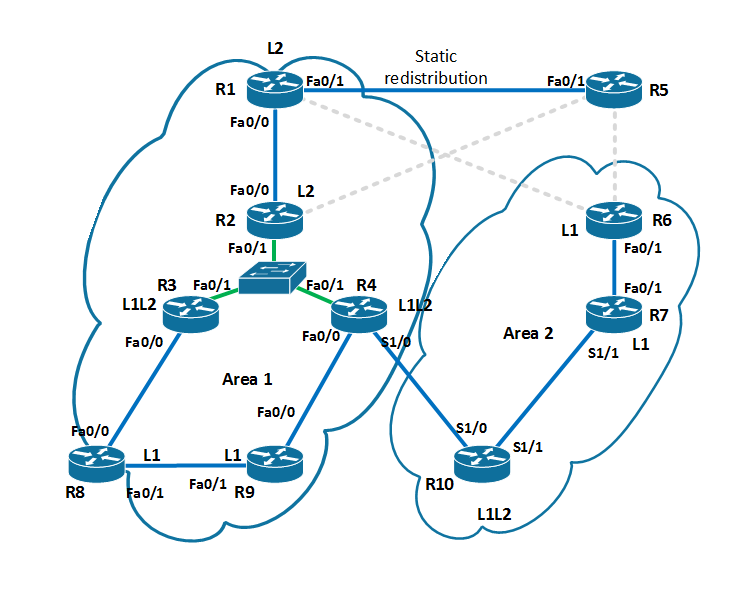
\includegraphics[width=12cm,keepaspectratio]{isis_topo}
\caption{Topológia IS-IS}
\label{fig:isis_topo}
\end{figure}



\begin{table}[!htb]
\centering
\caption{IP adresácia}
\label{tab:ip_adresacia}
\begin{tabular}{|c|c|l|l|l|}
\hline
\multicolumn{1}{|c|}{\textbf{Smerovač}}    & \multicolumn{1}{c|}{\textbf{Funkcia}}                        & \multicolumn{1}{c|}{\textbf{Rozhranie}} & \multicolumn{1}{c|}{\textbf{IP adresa}} & \multicolumn{1}{c|}{\textbf{Maska}} \\ \hline
\multirow{3}{*}{R1}  & \multirow{3}{*}{L2}                   & Fa0/0                                   & 10.0.12.1                               & 255.255.255.0                       \\ \cline{3-5} 
                     &                                         & Fa0/1                                   & 10.100.15.1                             & 255.255.255.0                       \\ \cline{3-5} 
                     &                                         & Lo0                                     & 10.255.255.1                            & 255.255.255.255                     \\ \hline
\multirow{3}{*}{R2}  & \multirow{3}{*}{L2}             & Fa0/0                                   & 10.0.12.2                               & 255.255.255.0                       \\ \cline{3-5} 
                     &                                         & Fa0/1                                   & 10.100.234.2                             & 255.255.255.0                       \\ \cline{3-5}
                     &                                         & Lo0                                     & 10.255.255.2                            & 255.255.255.255                     \\ \hline
\multirow{4}{*}{R3}  & \multirow{4}{*}{L1/L2}                    & Fa0/0                                   & 10.1.38.3                               & 255.255.255.0                       \\ \cline{3-5} 
                     &                                         & Fa0/1                                   & 10.0.234.3                              & 255.255.255.0                       \\ \cline{3-5} 
                     &                                         & S1/0                                    & 10.2.39.3                               & 255.255.255.252                     \\ \cline{3-5} 
                     &                                         & Lo0                                     & 10.255.255.3                            & 255.255.255.255                     \\ \hline
\multirow{4}{*}{R4}  & \multirow{4}{*}{L1/L2}                    & Fa0/0                                   & 10.2.49.4                               & 255.255.255.0                       \\ \cline{3-5} 
                     &                                         & Fa0/1                                   & 10.0.234.4                              & 255.255.255.0                       \\ \cline{3-5} 
                     &                                         & S1/0                                    & 10.3.104.4                              & 255.255.255.252                     \\ \cline{3-5} 
                     &                                         & Lo0                                     & 10.255.255.4                            & 255.255.255.255                     \\ \hline
\multirow{2}{*}{R5}  & \multirow{2}{*}{Smerovač iného systému} & Fa0/1                                   & 10.100.15.5                             & 255.255.255.0                       \\ \cline{3-5} 
                     &                                         & Lo0                                     & 10.255.255.5                            & 255.255.255.255                     \\ \hline
\multirow{2}{*}{R6}  & \multirow{2}{*}{L1}             & Fa0/0                                   & 10.4.67.6                               & 255.255.255.0                       \\ \cline{3-5} 
                     &                                         & Lo0                                     & 10.255.255.6                            & 255.255.255.255                     \\ \hline
\multirow{3}{*}{R7}  & \multirow{3}{*}{L1}             & Fa0/1                                   & 10.4.67.7                               & 255.255.255.0                       \\ \cline{3-5} 
                     &                                         & S1/1                                    & 10.4.107.7                              & 255.255.255.0                       \\ \cline{3-5} 
                     &                                         & Lo0                                     & 10.255.255.7                            & 255.255.255.255                     \\ \hline
\multirow{2}{*}{R8}  & \multirow{2}{*}{L1}             & Fa0/0                                   & 10.1.38.8                               & 255.255.255.0                       \\ \cline{3-5} 
                     &                                         & Lo0                                     & 10.255.255.8                            & 255.255.255.255                     \\ \hline
\multirow{3}{*}{R9}  & \multirow{3}{*}{L1}             & Fa0/0                                   & 10.2.49.9                               & 255.255.255.0                       \\ \cline{3-5} 
                     &                                         & S1/0                                    & 10.2.39.9                               & 255.255.255.0                       \\ \cline{3-5} 
                     &                                         & Lo0                                     & 10.255.255.9                            & 255.255.255.255                     \\ \hline
\multirow{3}{*}{R10} & \multirow{3}{*}{L1/L2}                    & S1/0                                    & 10.3.104.10                              & 255.255.255.0                       \\ \cline{3-5} 
                     &                                         & S1/1                                    & 10.4.107.10                              & 255.255.255.0                       \\ \cline{3-5} 
                     &                                         & Lo0                                     & 10.255.255.10                           & 255.255.255.255                     \\ \hline
\end{tabular}
\end{table}


% Novu kapitolu davam na novu stranu, lebo bez toho mi zobrazuje tabulku v dalsej kapitole, kde ale tabulka nepatri.
\newpage


\section{Úlohy}
\subsection{Základná konfigurácia}
\subsection{Nakonfigurovať IS-IS s dvoma oblasťami}
\subsection{R2, R3, R4 broadcast spojenia prostredníctvom L2 prepínača zvyšok spojení P2P}
\subsection{Router id – ISO NSAP formát odvodený z loopback0 rozhrania}
\subsubsection{Popis}
\paragraph{}
Ako za základnú konfiguráciu považujeme nastavenie adresácie, vzdialeného prístupu a vypisovania konzoly. IP adresy sme vytvárali tak, že prvý oktet bola 10, druhý oktet bolo číslo oblasti, tretí oktet bolo číslo, ktoré vzniklo ako spojenie čísel dvojíc smerovačov, medzi ktorými sa sieť nachádzala; napr. sieť medzi smerovačmi 4 a 10 by bol tretí oktet 104, medzi smerovačmi R1 a R2 by to bolo 12 atď. a štvrtý oktet bolo zvolené číslo smerovača.

\paragraph{}
ISO NSAP Router ID bolo odvodené od loopback0 rozhrania. Postup vytvorenia Router ID pre smerovač R1 uvádzame nižšie.

Postup vytvorenia ISO NSAP identifikátora:

\begin{enumerate}
\item Vezmeme IP adresu loopback0 rozhrania.
\noindent
{\fontfamily{qcr}\selectfont
\begin{small}
\begin{verbatim}
10.255.255.1
\end{verbatim}
\end{small}
}


\item Ak má oktet menej ako 3 cifry, vyplníme ho zľava nulami.
\noindent
{\fontfamily{qcr}\selectfont
\begin{small}
\begin{verbatim}
010.255.255.001
\end{verbatim}
\end{small}
}

\item Odstránime bodky.
\noindent
{\fontfamily{qcr}\selectfont
\begin{small}
\begin{verbatim}
010255255001
\end{verbatim}
\end{small}
}

\item Číslo rozdelíme po 4 cifrách
\noindent
{\fontfamily{qcr}\selectfont
\begin{small}
\begin{verbatim}
0102.5525.5001
\end{verbatim}
\end{small}
}

\item Ku koncu pripojíme NSEL (Network-Selector). \say{Selector} je pre naše účely 2 nuly. NSEL sa obvykle nepoužíva a mal by byť vyplnený nulami.
\noindent
{\fontfamily{qcr}\selectfont
\begin{small}
\begin{verbatim}
0102.5525.5001.00
\end{verbatim}
\end{small}
}

\item Na začiatok pridáme štvorciferný identifikátor oblasti, do ktorej smerovač patrí.
\noindent
{\fontfamily{qcr}\selectfont
\begin{small}
\begin{verbatim}
0001.0102.5525.5001.00
\end{verbatim}
\end{small}
}


\item Na začiatok pridáme AFI (Authority and Format Identifier), V našom prípade bude mať hodnotu \say{49}, čo znamená, že identifikátor patrí do privátneho rozsahu.
\noindent
{\fontfamily{qcr}\selectfont
\begin{small}
\begin{verbatim}
49.0001.0102.5525.5001.00
\end{verbatim}
\end{small}
}
\end{enumerate}

\paragraph{}
Takto vytvorený NSAP identifikátor je hotový a použiteľný na konfiguráciu.


\subsubsection{Konfigurácia}
\noindent
{\fontfamily{qcr}\selectfont
\begin{small}
\begin{verbatim}
!R1
ena
conf t
hostname R1
no ip domain-lookup
username admin privil 15 secret admin
line con 0
  login local
  logging syn
  exec-time 120
line vty 0 15
  privilege level 15
  no login
int f0/0
  ip addr 10.1.12.1 255.255.255.0
  ip router isis
  isis network point-to-point
  no shut
int lo0
  ip addr 10.255.255.1 255.255.255.255
  ip router isis
  no shut
int f0/1
  ip addr 10.100.15.1 255.255.255.0
  no shut
router isis
  net 49.0001.0102.5525.5001.00
  passive-interface lo0
  is-type level-2
  metric-style wide



!R2
ena
conf t
hostname R2
no ip domain-lookup
username admin privil 15 secret admin
line con 0
  login local
  logging syn
  exec-time 120
line vty 0 15
  privilege level 15
  no login
int f0/0
  ip addr 10.1.12.2 255.255.255.0
  ip router isis
  isis network point-to-point
  no shut
int lo0
  ip addr 10.255.255.2 255.255.255.255
  ip router isis
  no shut
int f0/1
  ip addr 10.1.234.2 255.255.255.0
  ip router isis
  no shut
router isis
  net 49.0001.0102.5525.5002.00
  passive-interface lo0
  is-type level-2
  metric-style wide




!R3
ena
conf t
hostname R3
no ip domain-lookup
username admin privil 15 secret admin
line con 0
  login local
  logging syn
  exec-time 120
line vty 0 15
  privilege level 15
  no login
int f0/0
  ip addr 10.1.38.3 255.255.255.0
  ip router isis
  isis network point-to-point
  no shut
int lo0
  ip addr 10.255.255.3 255.255.255.255
  ip router isis
  no shut
int f0/1
  ip addr 10.1.234.3 255.255.255.0
  ip router isis
  no shut
router isis
  net 49.0001.0102.5525.5003.00
  passive-interface lo0
  is-type level-1-2
  metric-style wide



!R4
ena
conf t
hostname R4
no ip domain-lookup
username admin privil 15 secret admin
line con 0
  login local
  logging syn
  exec-time 120
line vty 0 15
  privilege level 15
  no login
int f0/0
  ip addr 10.1.49.4 255.255.255.0
  ip router isis
  isis network point-to-point
  no shut
int lo0
  ip addr 10.255.255.4 255.255.255.255
  ip router isis
  no shut
int f0/1
  ip addr 10.1.234.4 255.255.255.0
  ip router isis
  no shut
int s1/0
  ip addr 10.1.104.4 255.255.255.0
  ip router isis
  no shut
router isis
  net 49.0001.0102.5525.5004.00
  passive-interface lo0
  is-type level-1-2
  metric-style wide



!R5
ena
conf t
hostname R5
no ip domain-lookup
username admin privil 15 secret admin
line con 0
  login local
  logging syn
  exec-time 120
line vty 0 15
  privilege level 15
  no login
int lo0
  ip addr 10.255.255.5 255.255.255.255
  no shut
int f0/1
  ip addr 10.100.15.5 255.255.255.0
  no shut




!R6
ena
conf t
hostname R6
no ip domain-lookup
username admin privil 15 secret admin
line con 0
  login local
  logging syn
  exec-time 120
line vty 0 15
  privilege level 15
  no login
int f0/1
  ip addr 10.2.67.6 255.255.255.0
  ip router isis
  isis network point-to-point
  no shut
int lo0
  ip addr 10.255.255.6 255.255.255.255
  ip router isis
  no shut
router isis
  net 49.0002.0102.5525.5006.00
  passive-interface lo0
  is-type level-1
  metric-style wide



!R7
ena
conf t
hostname R7
no ip domain-lookup
username admin privil 15 secret admin
line con 0
  login local
  logging syn
  exec-time 120
line vty 0 15
  privilege level 15
  no login
int f0/1
  ip addr 10.2.67.7 255.255.255.0
  ip router isis
  isis network point-to-point
  no shut
int lo0
  ip addr 10.255.255.7 255.255.255.255
  ip router isis
  no shut
int s1/1
  ip addr 10.2.107.7 255.255.255.0
  Ip router isis
  no shut
router isis
  net 49.0002.0102.5525.5007.00
  passive-interface lo0
  is-type level-1
  metric-style wide




!R8
ena
conf t
hostname R8
no ip domain-lookup
username admin privil 15 secret admin
line con 0
  login local
  logging syn
  exec-time 120
line vty 0 15
  privilege level 15
  no login
int f0/0
  ip addr 10.1.38.8 255.255.255.0
  ip router isis
  isis network point-to-point
  no shut
int lo0
  ip addr 10.255.255.8 255.255.255.255
  ip router isis
  no shut
int f0/1
  ip addr 10.1.89.8 255.255.255.0
  Ip router isis
  isis network point-to-point
  no shut
router isis
  net 49.0001.0102.5525.5008.00
  passive-interface lo0
  is-type level-1
  metric-style wide




!R9
ena
conf t
hostname R9
no ip domain-lookup
username admin privil 15 secret admin
line con 0
  login local
  logging syn
  exec-time 120
line vty 0 15
  privilege level 15
  no login
int f0/0
  ip addr 10.1.49.9 255.255.255.0
  ip router isis
  isis network point-to-point
  no shut
int lo0
  ip addr 10.255.255.9 255.255.255.255
  ip router isis
  no shut
int f0/1
  ip addr 10.1.89.9 255.255.255.0
  Ip router isis
  isis network point-to-point
  no shut
router isis
  net 49.0001.0102.5525.5009.00
  passive-interface lo0
  is-type level-1
  metric-style wide




!R10
ena
conf t
hostname R10
no ip domain-lookup
username admin privil 15 secret admin
line con 0
  login local
  logging syn
  exec-time 120
line vty 0 15
  privilege level 15
  no login
int s1/0
  ip addr 10.1.104.10 255.255.255.0
  ip router isis
  no shut
int lo0
  ip addr 10.255.255.10 255.255.255.255
  ip router isis
  no shut
int s1/1
  ip addr 10.2.107.10 255.255.255.0
  Ip router isis
  no shut
router isis
  net 49.0002.0102.5525.5010.00
  passive-interface lo0
  is-type level-1-2
  metric-style wide
\end{verbatim}
\end{small}
}

\subsubsection{Overenie}
\paragraph{}
Základnú konfiguráciu sme overili príkazmi \say{show ip interface brief}. Nižšie je uvedený výpis zo smerovača R1. Router ID sme overili príkazom \say{show isis hostname}. DIS smerovač sme overili príkazom \say{show isis database}. Bližšie vysvetlenie DIS smerovača sa nachádza v kapitole ~\ref{kontrola_lan_dis} \nameref{kontrola_lan_dis}.

\noindent
{\fontfamily{qcr}\selectfont
\begin{small}
\begin{verbatim}

R1#show ip int b
Interface                  IP-Address      OK? Method Status   Protocol
FastEthernet0/0            10.1.12.1       YES manual up       up      
FastEthernet0/1            10.100.15.1     YES manual up       up      
...    
Loopback0                  10.255.255.1    YES manual up       up  

\end{verbatim}
\end{small}
}

\noindent
{\fontfamily{qcr}\selectfont
\begin{small}
\begin{alltt}

R1#show isis hostname
Level  System ID      Dynamic Hostname  (notag)
 2     0102.5525.5003 R3
 2     0102.5525.5002 R2
     * 0102.5525.5001 R1
 2     0102.5525.5004 R4
 2     0102.5525.5010 R10

\end{alltt}
\end{small}
}

\noindent
{\fontfamily{qcr}\selectfont
\begin{small}
\begin{alltt}
R1#show isis database

IS-IS Level-2 Link State Database:
LSPID                 LSP Seq Num  LSP Checksum  LSP Holdtime      ATT/P/OL
R1.00-00            * 0x0000000B   0x937D        1031              0/0/0
R2.00-00              0x0000000A   0xB628        852               0/0/0
R2.01-00              0x00000009   0x5821        901               0/0/0
R3.00-00              0x0000000D   0xA6AA        681               0/0/0
R4.00-00              0x0000000D   0xF394        764               0/0/0
R10.00-00             0x0000000B   0xA9D4        846               0/0/0
\end{alltt}
\end{small}
}

\paragraph{}
Z výpisu príkazu \say{show ip interface brief} je zrejmé, že IP adresy boli nastavené. Z výpisu príkazu \say{show isis hostname} vieme, že identifikátory smerovačov sú správne nastavené k prislúchajúcim názvom smerovačov. Vidíme mená iba tých smerovačov, s ktorými má R1 založený L2 vzťah. Vo výpise \say{show isis database} vidíme, že v broadcastovej doméne medzi smerovačmi R2, R3 a R4 bol za DIS zvolený smerovač R4. Spoznáme to podľa nenulovej prvej dvojice čísel hneď za názvom smerovača \say{R4.\textbf{\textit{02}}-00}.



\subsection{Statická redistribúcia smerovacích záznamov z R5}
\subsubsection{Popis}
\paragraph{}
Smerovač R5 bolo potrebné prepojiť ku IS-IS topológií tým, že staticky nastavíme cestu z R1 na R5 a v.v., ktorú R1 prepošle medzi všetky IS-IS smerovače.

\subsubsection{Konfigurácia}
\noindent
{\fontfamily{qcr}\selectfont
\begin{small}
\begin{verbatim}
R5(config)#ip route 0.0.0.0 0.0.0.0 f0/1 10.100.15.1

R1(config)#ip route 10.255.255.5 255.255.255.255 f0/1 10.100.15.5
R1(config)#router isis
R1(config-router)#redistribute static
R1(config-router)#redistribute connected
\end{verbatim}
\end{small}
}

\subsubsection{Overenie}
\paragraph{}
Konfiguráciu statickej cesty sme overili príkazom \say{show ip route} na smerovačoch R5, R1 a R2 (v takomto poradí).

\paragraph{}
Výpis smerovacej tabuľky z R5:

\noindent
{\fontfamily{qcr}\selectfont
\begin{small}
\begin{alltt}
R5#show ip route
...
Gateway of last resort is 0.0.0.0 to network 0.0.0.0

     10.0.0.0/8 is variably subnetted, 2 subnets, 2 masks
C       10.255.255.5/32 is directly connected, Loopback0
C       10.100.15.0/24 is directly connected, FastEthernet0/1
S*   0.0.0.0/0 is directly connected, FastEthernet0/1
\end{alltt}
\end{small}
}

\paragraph{}
Výpis smerovacej tabuľky z R1:

\noindent
{\fontfamily{qcr}\selectfont
\begin{small}
\begin{alltt}
R1#show ip route
Gateway of last resort is 10.100.15.5 to network 0.0.0.0

     10.0.0.0/8 is variably subnetted, 19 subnets, 2 masks
...
S       10.255.255.5/32 [1/0] via 10.100.15.5, FastEthernet0/1
...
C       10.100.15.0/24 is directly connected, FastEthernet0/1
...
S*   0.0.0.0/0 [1/0] via 10.100.15.5, FastEthernet0/1
\end{alltt}
\end{small}
}

\paragraph{}
Výpis smerovacej tabuľky z R2:

\noindent
{\fontfamily{qcr}\selectfont
\begin{small}
\begin{alltt}
R2#show ip route
...
Gateway of last resort is not set
...
i L2    10.255.255.5/32 [115/10] via 10.1.12.1, FastEthernet0/0
...
i L2    10.100.15.0/24 [115/10] via 10.1.12.1, FastEthernet0/0
...
\end{alltt}
\end{small}
}

\paragraph{}
Z výpisov smerovacích tabuliek vyplýva, že smerovač R5 má nastavenú predvolenú cestu staticky ku R1, ktorú potom rozšíri do zvyšku IS-IS topológie.





\subsection{R3 – R4 P2P, L2 only}
\subsubsection{Popis}
\paragraph{}
Keďže R3 a R4 sú smerovače typu L1/L2, štandardne sa medzi nimi vytvorí L1 aj L2 spojenie. Bolo potrebné nastaviť, aby spojenie medzi smerovačmi R3 a R4 bolo iba typu L2.

\subsubsection{Konfigurácia}
\paragraph{}
Na smerovačoch R3 a R4 vykonáme tieto príkazy:

\noindent
{\fontfamily{qcr}\selectfont
\begin{small}
\begin{verbatim}
int f0/1
  isis circuit-type level-2
\end{verbatim}
\end{small}
}

\subsubsection{Overenie}
\paragraph{}
Susedstvo sme overovali príkazom \say{}.

\noindent
{\fontfamily{qcr}\selectfont
\begin{small}
\begin{alltt}
R3#show isis neighbors

System Id      Type Interface   IP Address      State Holdtime Circuit Id
R8             L1   Fa0/0       10.1.38.8       UP    24       00
\textbf{R4             L2   Fa0/1       10.1.234.4      UP    27       R2.01}
R2             L2   Fa0/1       10.1.234.2      UP    8        R2.01
\end{alltt}
\end{small}
}

\paragraph{}
Z výpisu vyplýva, že medzi smerovačmi R3 a R4 bolo vytvorené iba L2 susedstvo.






\subsection{Kontrola LAN DIS}
\label{kontrola_lan_dis}
\subsubsection{Popis}
\paragraph{}
Medzi smerovačmi R2, R3 a R4 musel byť zvolený DIS (Designated Intermediate System). DIS je virtuálny smerovač, ktorý plní rovnakú funkciu ako DR (Designated Router) v OSPF: zvolí sa jeden smerovač, ktorý si udržuje spojenia so všetkými ostatnými smerovačmi v broadcastovej doméne. Tým sa znižuje výpočtové zaťaženie a zmenšuje veľkosť IS-IS databázy na smerovačoch v broadcastovej doméne, pretože si nemusia posielať správy každý s každým, čo bz vyúsťovalo do faktoriálovej zložitosti. Namiesto toho každý smerovač udržuje spojenie iba s DIS smerovačom, ktorý následne podľa potreby preposiela správy iným smerovačom v broadcastovej doméne. IS-IS, narozdiel od OSPF, nemá ekvivalent BDR t.j. v IS-IS neexistuje záložný DIS smerovač.

\paragraph{}
Dohodli sme sa, že DIS bude na smerovači R2. Predvolená priorita pre smerovače je 64. Platí, že čím vyššie číslo, tým vyššia priorita. Voľba DIS smerovača v IS-IS je preemptívna, čo znamená že  po nastavení priority prebehne voľba DIS smerovača narozdiel od OSPF, kde voľba musela byť vykonaná zmenou priority a následným reštartom OSPF procesu.

\subsubsection{Konfigurácia}
\paragraph{}
Na smerovači R2 vykonáme tieto príkazy:
\noindent
{\fontfamily{qcr}\selectfont
\begin{small}
\begin{verbatim}
int f0/1
  isis priority 100
\end{verbatim}
\end{small}
}

\subsubsection{Overenie}
\paragraph{}
Konfiguráciu sme overili príkazmi \say{show clns interface f0/1} a \say{show isis database} na smerovači R2.

\paragraph{}
Výpisy pred zmenou DIS z R2:

\noindent
{\fontfamily{qcr}\selectfont
\begin{small}
\begin{alltt}
R2#show clns int f0/1
FastEthernet0/1 is up, line protocol is up
  Checksums enabled, MTU 1497, Encapsulation SAP
  ERPDUs enabled, min. interval 10 msec.
  CLNS fast switching enabled
  CLNS SSE switching disabled
  DEC compatibility mode OFF for this interface
  Next ESH/ISH in 27 seconds
  Routing Protocol: IS-IS
    Circuit Type: level-1-2
    Interface number 0x1, local circuit ID 0x1
    Level-2 Metric: 10, \textbf{Priority: 64}, Circuit ID: R4.01
    DR ID: R4.01
    Level-2 IPv6 Metric: 10
    Number of active level-2 adjacencies: 2
    Next IS-IS LAN Level-2 Hello in 4 seconds


--------------------------------------------------------------------------


R2#show isis database

IS-IS Level-2 Link State Database:
LSPID                 LSP Seq Num  LSP Checksum  LSP Holdtime      ATT/P/OL
R1.00-00              0x00000010   0x8982        1082              0/0/0
R2.00-00            * 0x0000000F   0xE4F2        576               0/0/0
R3.00-00              0x00000012   0xE861        783               0/0/0
R4.00-00              0x00000012   0xC5BB        618               0/0/0
\textbf{R4.\textit{01}-00              0x00000002   0x403E        620               0/0/0}
R10.00-00             0x00000010   0x9FD9        1034              0/0/0

\end{alltt}
\end{small}
}

\paragraph{}
Ak je prvé dvojčíslie nulové (00), potom je to point-to-point linka, pretože sa nevolil DIS smerovač. Ak je nenulové, daný smerovač bol zvolený ako DIS. Pred zmenou bol za DIS zvolený smerovač R4.


\paragraph{}
Výpisy po zmene DIS na R2:

\noindent
{\fontfamily{qcr}\selectfont
\begin{small}
\begin{alltt}

R2#show clns int f0/1
FastEthernet0/1 is up, line protocol is up
  Checksums enabled, MTU 1497, Encapsulation SAP
  ERPDUs enabled, min. interval 10 msec.
  CLNS fast switching enabled
  CLNS SSE switching disabled
  DEC compatibility mode OFF for this interface
  Next ESH/ISH in 38 seconds
  Routing Protocol: IS-IS
    Circuit Type: level-1-2
    Interface number 0x1, local circuit ID 0x1
    Level-2 Metric: 10, \textbf{Priority: 100}, Circuit ID: R2.01
    DR ID: R2.01
    Level-2 IPv6 Metric: 10
    Number of active level-2 adjacencies: 2
    Next IS-IS LAN Level-2 Hello in 1 seconds


--------------------------------------------------------------------------


R2#show isis database

IS-IS Level-2 Link State Database:
LSPID                 LSP Seq Num  LSP Checksum  LSP Holdtime      ATT/P/OL
R1.00-00              0x00000010   0x8982        343               0/0/0
R2.00-00            * 0x00000011   0xA82F        1047              0/0/0
\textbf{R2.01-00            * 0x00000001   0x6819        1048              0/0/0}
R3.00-00              0x00000014   0x98B1        1045              0/0/0
R4.00-00              0x00000014   0xE59B        1045              0/0/0
\textit{R4.01-00              0x00000003   0xBF67        0 (1047)          0/0/0}
R10.00-00             0x00000011   0x9DDA        1039              0/0/0
\end{alltt}
\end{small}
}

\paragraph{}
Po zmene priority vidíme, že R4 už nie je DIS smerovač, pretože \say{LSP Holdtime} je vynulovaný. Záznam sa z databázy vymaže prejaví až po uplynutí času v zátvorke (v sekundách). Nižšie je uvedená finálna podoba IS-IS databázy.

\noindent
{\fontfamily{qcr}\selectfont
\begin{small}
\begin{alltt}
R2#show isis database

IS-IS Level-2 Link State Database:
LSPID                 LSP Seq Num  LSP Checksum  LSP Holdtime      ATT/P/OL
R1.00-00              0x00000012   0x8584        661               0/0/0
R2.00-00            * 0x00000012   0xA630        484               0/0/0
\textbf{R2.01-00            * 0x00000002   0x661A        494               0/0/0}
R3.00-00              0x00000016   0x94B3        1182              0/0/0
R4.00-00              0x00000015   0xE39C        470               0/0/0
R10.00-00             0x00000012   0x9BDB        540               0/0/0
\end{alltt}
\end{small}
}






\subsection{Area 2 – redistribúcia L2 do L1}
\subsubsection{Popis}
\paragraph{}
Redistribúcia smerovacích záznamov z L2 do L1 slúži na to, aby L1 smerovače v oblasti 2 videli cesty z L2 smerovačov v oblasti 1. Je to užitočné  robiť vtedy, ak chceme zabezpečiť optimálne smerovanie od L1 smerovačov. Aby takáto redistribúcia fungovala, musí byť na všetkých smerovačoch v IS-IS topológií nastavená rovnaká metrika; v našom prípade bola typu \say{wide}.

\subsubsection{Konfigurácia}
\paragraph{}
Konfigurujeme L1/L2 smerovač R10. Najprv si vytvoríme ACL, ktorý bude obsahovať všetky siete, ktoré chceme L1 smerovačom preposlať.

\noindent
{\fontfamily{qcr}\selectfont
\begin{small}
\begin{verbatim}
access-list 100 permit ip 10.255.255.1 0.0.0.0 any
access-list 100 permit ip 10.255.255.2 0.0.0.0 any
access-list 100 permit ip 10.255.255.3 0.0.0.0 any
access-list 100 permit ip 10.255.255.4 0.0.0.0 any
access-list 100 permit ip 10.1.12.0 0.0.0.255 any
access-list 100 permit ip 10.1.234.0 0.0.0.255 any
access-list 100 permit ip 10.1.38.0 0.0.0.255 any
access-list 100 permit ip 10.1.49.0 0.0.0.255 any

router isis
  metric-style wide
  redistribute isis ip level-2 into level-1 distribute-list 100
\end{verbatim}
\end{small}
}

\subsubsection{Overenie}
\paragraph{}
Konfiguráciu overíme príkazom \say{show ip route} na L1 smerovačoch v oblasti 2 (R6 alebo R7).

\noindent
{\fontfamily{qcr}\selectfont
\begin{small}
\begin{verbatim}

R6#show ip route
...
Gateway of last resort is 10.2.67.7 to network 0.0.0.0

     10.0.0.0/8 is variably subnetted, 14 subnets, 2 masks
i L1    10.255.255.10/32 [115/20] via 10.2.67.7, FastEthernet0/1
i ia    10.1.12.0/24 [115/50] via 10.2.67.7, FastEthernet0/1
i ia    10.255.255.2/32 [115/40] via 10.2.67.7, FastEthernet0/1
i ia    10.255.255.3/32 [115/40] via 10.2.67.7, FastEthernet0/1
i ia    10.255.255.1/32 [115/50] via 10.2.67.7, FastEthernet0/1
C       10.255.255.6/32 is directly connected, Loopback0
i L1    10.255.255.7/32 [115/10] via 10.2.67.7, FastEthernet0/1
i ia    10.255.255.4/32 [115/30] via 10.2.67.7, FastEthernet0/1
i ia    10.1.38.0/24 [115/50] via 10.2.67.7, FastEthernet0/1
i ia    10.1.49.0/24 [115/40] via 10.2.67.7, FastEthernet0/1
C       10.2.67.0/24 is directly connected, FastEthernet0/1
i L1    10.2.107.0/24 [115/20] via 10.2.67.7, FastEthernet0/1
i L1    10.1.104.0/24 [115/30] via 10.2.67.7, FastEthernet0/1
i ia    10.1.234.0/24 [115/40] via 10.2.67.7, FastEthernet0/1
i*L1 0.0.0.0/0 [115/20] via 10.2.67.7, FastEthernet0/1

\end{verbatim}
\end{small}
}

\paragraph{}
Výpis smerovacej tabuľky zo smerovača R6 ukazuje siete naučené z L2 smerovačov ako \say{ia} - Inter-Area IS-IS siete.





\subsection{R8, R9 – R3 primárny smerovač pre všetky vnútorné adresy}
\label{R8_primarny_smerovac}
\subsubsection{Popis}
\paragraph{}
Ďalej ovplyvňujeme smerovanie tak, že pre smerovače R8 a R9 budeme pre vnútorné adresy používať smerovač R3.


\subsubsection{Konfigurácia}
\paragraph{}
Na smerovači R9 sme zhoršili metriku aby bol R3 primárny smerovač pre všetky vnútorné adresy smerovačov R8 a R9

\noindent
{\fontfamily{qcr}\selectfont
\begin{small}
\begin{verbatim}

R9(config)#int f0/0
R9(config-if)#isis metric 100
\end{verbatim}
\end{small}
}

\subsubsection{Overenie}
\paragraph{}
show clns interface f0/0 (porovnať metriku rozhrania - predtým [10] a potom [100] )


\paragraph{}
Pred konfiguráciou:

\noindent
{\fontfamily{qcr}\selectfont
\begin{small}
\begin{alltt}
R8#traceroute 10.255.255.1

Type escape sequence to abort.
Tracing the route to 10.255.255.1

\textbf{  1 10.1.38.3 12 msec 16 msec 16 msec}
  2 10.1.234.2 36 msec 36 msec 36 msec
  3 10.1.12.1 56 msec *  72 msec



R9#traceroute 10.255.255.1

Type escape sequence to abort.
Tracing the route to 10.255.255.1

\textbf{  1 10.1.49.4 16 msec 16 msec 16 msec}
  2 10.1.234.2 32 msec 36 msec 40 msec
  3 10.1.12.1 68 msec *  52 msec

\end{alltt}
\end{small}
}

\paragraph{}
Vidíme, že z R8 ide smerovanie na vnútornú adresu cez R3, ale z R9 ide cez R4, pretože cesta cez R4 má menšiu metriku.



\paragraph{}
Po konfigurácií:

\noindent
{\fontfamily{qcr}\selectfont
\begin{small}
\begin{alltt}
R8#traceroute 10.255.255.1

Type escape sequence to abort.
Tracing the route to 10.255.255.1

\textbf{  1 10.1.38.3 8 msec 16 msec 16 msec}
  2 10.1.234.2 24 msec 36 msec 44 msec
  3 10.1.12.1 44 msec *  68 msec



R9#traceroute 10.255.255.1

Type escape sequence to abort.
Tracing the route to 10.255.255.1

  1 10.1.89.8 20 msec 16 msec 20 msec
\textbf{  2 10.1.38.3 40 msec 40 msec 40 msec}
  3 10.1.234.2 56 msec 36 msec 80 msec
  4 10.1.12.1 56 msec *  68 msec
\end{alltt}
\end{small}
}

\paragraph{}
Z výpisov príkazu \say{traceroute} z R8 a R9 na smerovač R5 vidíme, že pre vnútorné adresy používajú R8 a R9 smerovač R3.






\subsection{R4 primárny smerovač len pre R5 smerovacie záznamy}
\subsubsection{Popis}
\paragraph{}
Smerovanie ovplyvňujeme ešte tým, že pre smerovače R8 a R9 určíme, aby prevádzka smerom k R5 išla cez smerovač R4.

\subsubsection{Konfigurácia}
\paragraph{}
Na R4 vytvoríme ACL, v ktorom povolíme siete pripojené ku R5. Tie sa následne prepošlú smerovačom R8 a R9, ktoré budú používať R4 ako primárny smerovač len pre prevádzku určenú pre R5.

\noindent
{\fontfamily{qcr}\selectfont
\begin{small}
\begin{verbatim}
access-list 101 permit ip 10.255.255.5 0.0.0.0 any
access-list 101 permit ip 10.100.15.0 0.0.0.255 any
router isis
  redistribute isis ip level-2 into level-1 distribute-list 101

\end{verbatim}
\end{small}
}

\subsubsection{Overenie}
\paragraph{}
Konfiguráciu sme overovali príkazom \say{traceroute} na IP adresy 10.100.15.5 a 10.255.255.2, aby sme sa uistili, či sa cesty líšia.

\noindent
{\fontfamily{qcr}\selectfont
\begin{small}
\begin{alltt}
\textbf{R8#traceroute 10.100.15.5}

Type escape sequence to abort.
Tracing the route to 10.100.15.5

  1 10.1.89.9 8 msec 16 msec 16 msec
\textbf{  2 10.1.49.4 36 msec 36 msec 36 msec}
  3 10.1.234.2 56 msec 36 msec 80 msec
  4 10.1.12.1 56 msec 88 msec 68 msec
  5 10.100.15.5 108 msec *  * 




\textbf{R8#traceroute 10.255.255.2}

Type escape sequence to abort.
Tracing the route to 10.255.255.2

\textbf{  1 10.1.38.3 16 msec 16 msec 16 msec}
  2 10.1.234.2 28 msec *  16 msec


--------------------------------------------------------------------------


\textbf{R9#traceroute 10.100.15.5}

Type escape sequence to abort.
Tracing the route to 10.100.15.5

\textbf{  1 10.1.49.4 16 msec 16 msec 20 msec}
  2 10.1.234.2 24 msec 36 msec 44 msec
  3 10.1.12.1 64 msec 48 msec 68 msec
  4 10.100.15.5 60 msec *  80 msec




\textbf{R9#traceroute 10.255.255.2}

Type escape sequence to abort.
Tracing the route to 10.255.255.2

  1 10.1.89.8 16 msec 16 msec 20 msec
\textbf{  2 10.1.38.3 24 msec 36 msec 40 msec}
  3 10.1.234.2 64 msec *  64 msec


--------------------------------------------------------------------------


R5#traceroute 10.255.255.8

Type escape sequence to abort.
Tracing the route to 10.255.255.8

  1 10.100.15.1 8 msec 16 msec 20 msec
  2 10.1.12.2 36 msec 36 msec 36 msec
  3 10.1.234.3 60 msec 36 msec 76 msec
  4 10.1.38.8 88 msec *  80 msec
R5#traceroute 10.255.255.9

Type escape sequence to abort.
Tracing the route to 10.255.255.9

  1 10.100.15.1 16 msec 16 msec 16 msec
  2 10.1.12.2 28 msec 40 msec 36 msec
  3 10.1.234.4 72 msec 44 msec 68 msec
  4 10.1.49.9 56 msec *  64 msec


--------------------------------------------------------------------------


R2#show ip route
...
Gateway of last resort is not set

     10.0.0.0/8 is variably subnetted, 19 subnets, 2 masks
...
\textbf{i L2    10.255.255.8/32 [115/20] via 10.1.234.3, FastEthernet0/1}
\textbf{i L2    10.255.255.9/32 [115/20] via 10.1.234.4, FastEthernet0/1}
\end{alltt}
\end{small}
}

\paragraph{}
Zo smerovačov R8 aj R9 ide smerovanie na R5 cez R4, ale z R5 na R8 nejde cez R4 ale cez bližší router R3, pretože tak hovorila smerovacia tabuľka na R2. Z R5 na R9 išlo smerovanie rovnako cez R4 (takisto kvôli smerovacej tabuľke na R2).





\subsection{Skrátenie hello a dead–interval časovačov, zistenie funkčnosti vytrhnutím jednej z liniek smerom ku L2 prepínaču}
\subsubsection{Popis}
\paragraph{}
\say{Hello} je predvolene nastavený na 10s a \say{dead} interval je 3-násobok \say{hello}. \say{Dead} interval sa nastavuje cez multiplikátor. My sme skrátili \say{hello} interval na 2s. \say{Hello} a \say{dead} intervaly sme menili iba na smerovačoch v broadcastovej doméne.


\subsubsection{Konfigurácia}
Na smerovačoch R2, R3 a R4 vykonáme tieto príkazy.

\noindent
{\fontfamily{qcr}\selectfont
\begin{small}
\begin{verbatim}

int f0/1
  isis hello-interval 3 level-1
  isis hello-interval 3 level-2


\end{verbatim}
\end{small}
}

\subsubsection{Overenie}
\paragraph{}
Na jednom zo smerovačov vykonáme v privilegovanom režime príkaz \say{debug isis adj-packets}. Sledujeme časy odosielania ‘sending’ správ. Tie budú chodiť v pravidelných intervaloch t.j. každé 3 sekundy. Nižšie je uvedený výpis príkazu \say{debug isis adj-packets} zo smerovača R2.

\noindent
{\fontfamily{qcr}\selectfont
\begin{small}
\begin{alltt}
...
\textbf{*Mar 13 04:15:24.691: ISIS-Adj: Rec L2 IIH from c021.025d.0001 \\(FastEthernet0/1), cir type L2, cir id 0102.5525.5002.01, length 1497}
...
\textbf{*Mar 13 04:15:27.675: ISIS-Adj: Rec L2 IIH from c021.025d.0001 \\(FastEthernet0/1), cir type L2, cir id 0102.5525.5002.01, length 1497}
...
\end{alltt}
\end{small}
}

\paragraph{}
Z \say{debug} výpisu vidíme, že \say{hello} pakety sa posielajú každé 3 sekundy na porte \say{Fa0/1}.


\subsection{Status linky R4 – R10 ? L1L2 ?}
\subsubsection{Popis}
\paragraph{}
Skontrolujeme stav linky medzi smerovačmi na rozhraní oblastí t.j. medzi R4 a R10.

\subsubsection{Overenie}
\paragraph{}
Stav linky sme overili príkazom \say{show clns interface s1/0} na smerovačoch R4 a R10.

\noindent
{\fontfamily{qcr}\selectfont
\begin{small}
\begin{alltt}
R4#show clns interface s1/0
Serial1/0 is up, line protocol is up
  Checksums enabled, MTU 1500, Encapsulation HDLC
  ERPDUs enabled, min. interval 10 msec.
  CLNS fast switching enabled
  CLNS SSE switching disabled
  DEC compatibility mode OFF for this interface
  Next ESH/ISH in 8 seconds
  Routing Protocol: IS-IS
    \textbf{Circuit Type: level-1-2}
    Interface number 0x2, local circuit ID 0x101
    Neighbor System-ID: R10
    Level-1 Metric: 10, Priority: 64, Circuit ID: R10.00
    Level-1 IPv6 Metric: 10
    Number of active level-1 adjacencies: 0
    Level-2 Metric: 10, Priority: 64, Circuit ID: R4.01
    Level-2 IPv6 Metric: 10
    Number of active level-2 adjacencies: 1
    Next IS-IS Hello in 3 seconds
    if state UP


--------------------------------------------------------------------------


R10#show clns interface s1/0
Serial1/0 is up, line protocol is up
  Checksums enabled, MTU 1500, Encapsulation HDLC
  ERPDUs enabled, min. interval 10 msec.
  CLNS fast switching enabled
  CLNS SSE switching disabled
  DEC compatibility mode OFF for this interface
  Next ESH/ISH in 44 seconds
  Routing Protocol: IS-IS
    \textbf{Circuit Type: level-1-2}
    Interface number 0x0, local circuit ID 0x100
    Neighbor System-ID: R4
    Level-1 Metric: 10, Priority: 64, Circuit ID: R10.00
    Level-1 IPv6 Metric: 10
    Number of active level-1 adjacencies: 0
    Level-2 Metric: 10, Priority: 64, Circuit ID: R10.00
    Level-2 IPv6 Metric: 10
    Number of active level-2 adjacencies: 1
    Next IS-IS Hello in 5 seconds
    if state UP
\end{alltt}
\end{small}
}

\paragraph{}
V obidvoch výpisoch vidíme, že \say{Circuit Type} je typu L1 aj L2 (level-1-2).


\end{document}